\chapter{Exp5: Pushing task with pose estimation from LIDAR}

This aim of this experiment was originally to show that a policy could be
learned on real robots for pushing a cube to some target pose. However,
experiments in simulation were harder than anticipated and consumed several
weeks before solving the problem. Also, when adding the same amount of noise
expected to come from sensors to the simulation problem, it failed to converge
to any decent policy. The policy trained in the non-noisy simulation worked
quite well when applied to the real setup which is described in more detail
below.

\section{Method}

To estimate the pose of the cube, a LIDAR was used by placing it in front of
the robot arm (figure \ref{fig:eef-frame}). The cube to push was a red wooden
cube with all sides measuring $4$ cm. One of these sides can be found from the
LIDAR-measurements by plotting the points onto a matrix/image and using the
Hough transform \cite{duda1972use}, see section \ref{sec:method_hough}. For the following experiments, only the
position of the cube was kept, ignoring the rotation. Conversion of the found
position of the cube to robot-frame was done using a least-squares approach
after randomly placing the cube at several positions known from the
forward-kinematics of the arm.

\begin{figure}[h!]
    \centering
    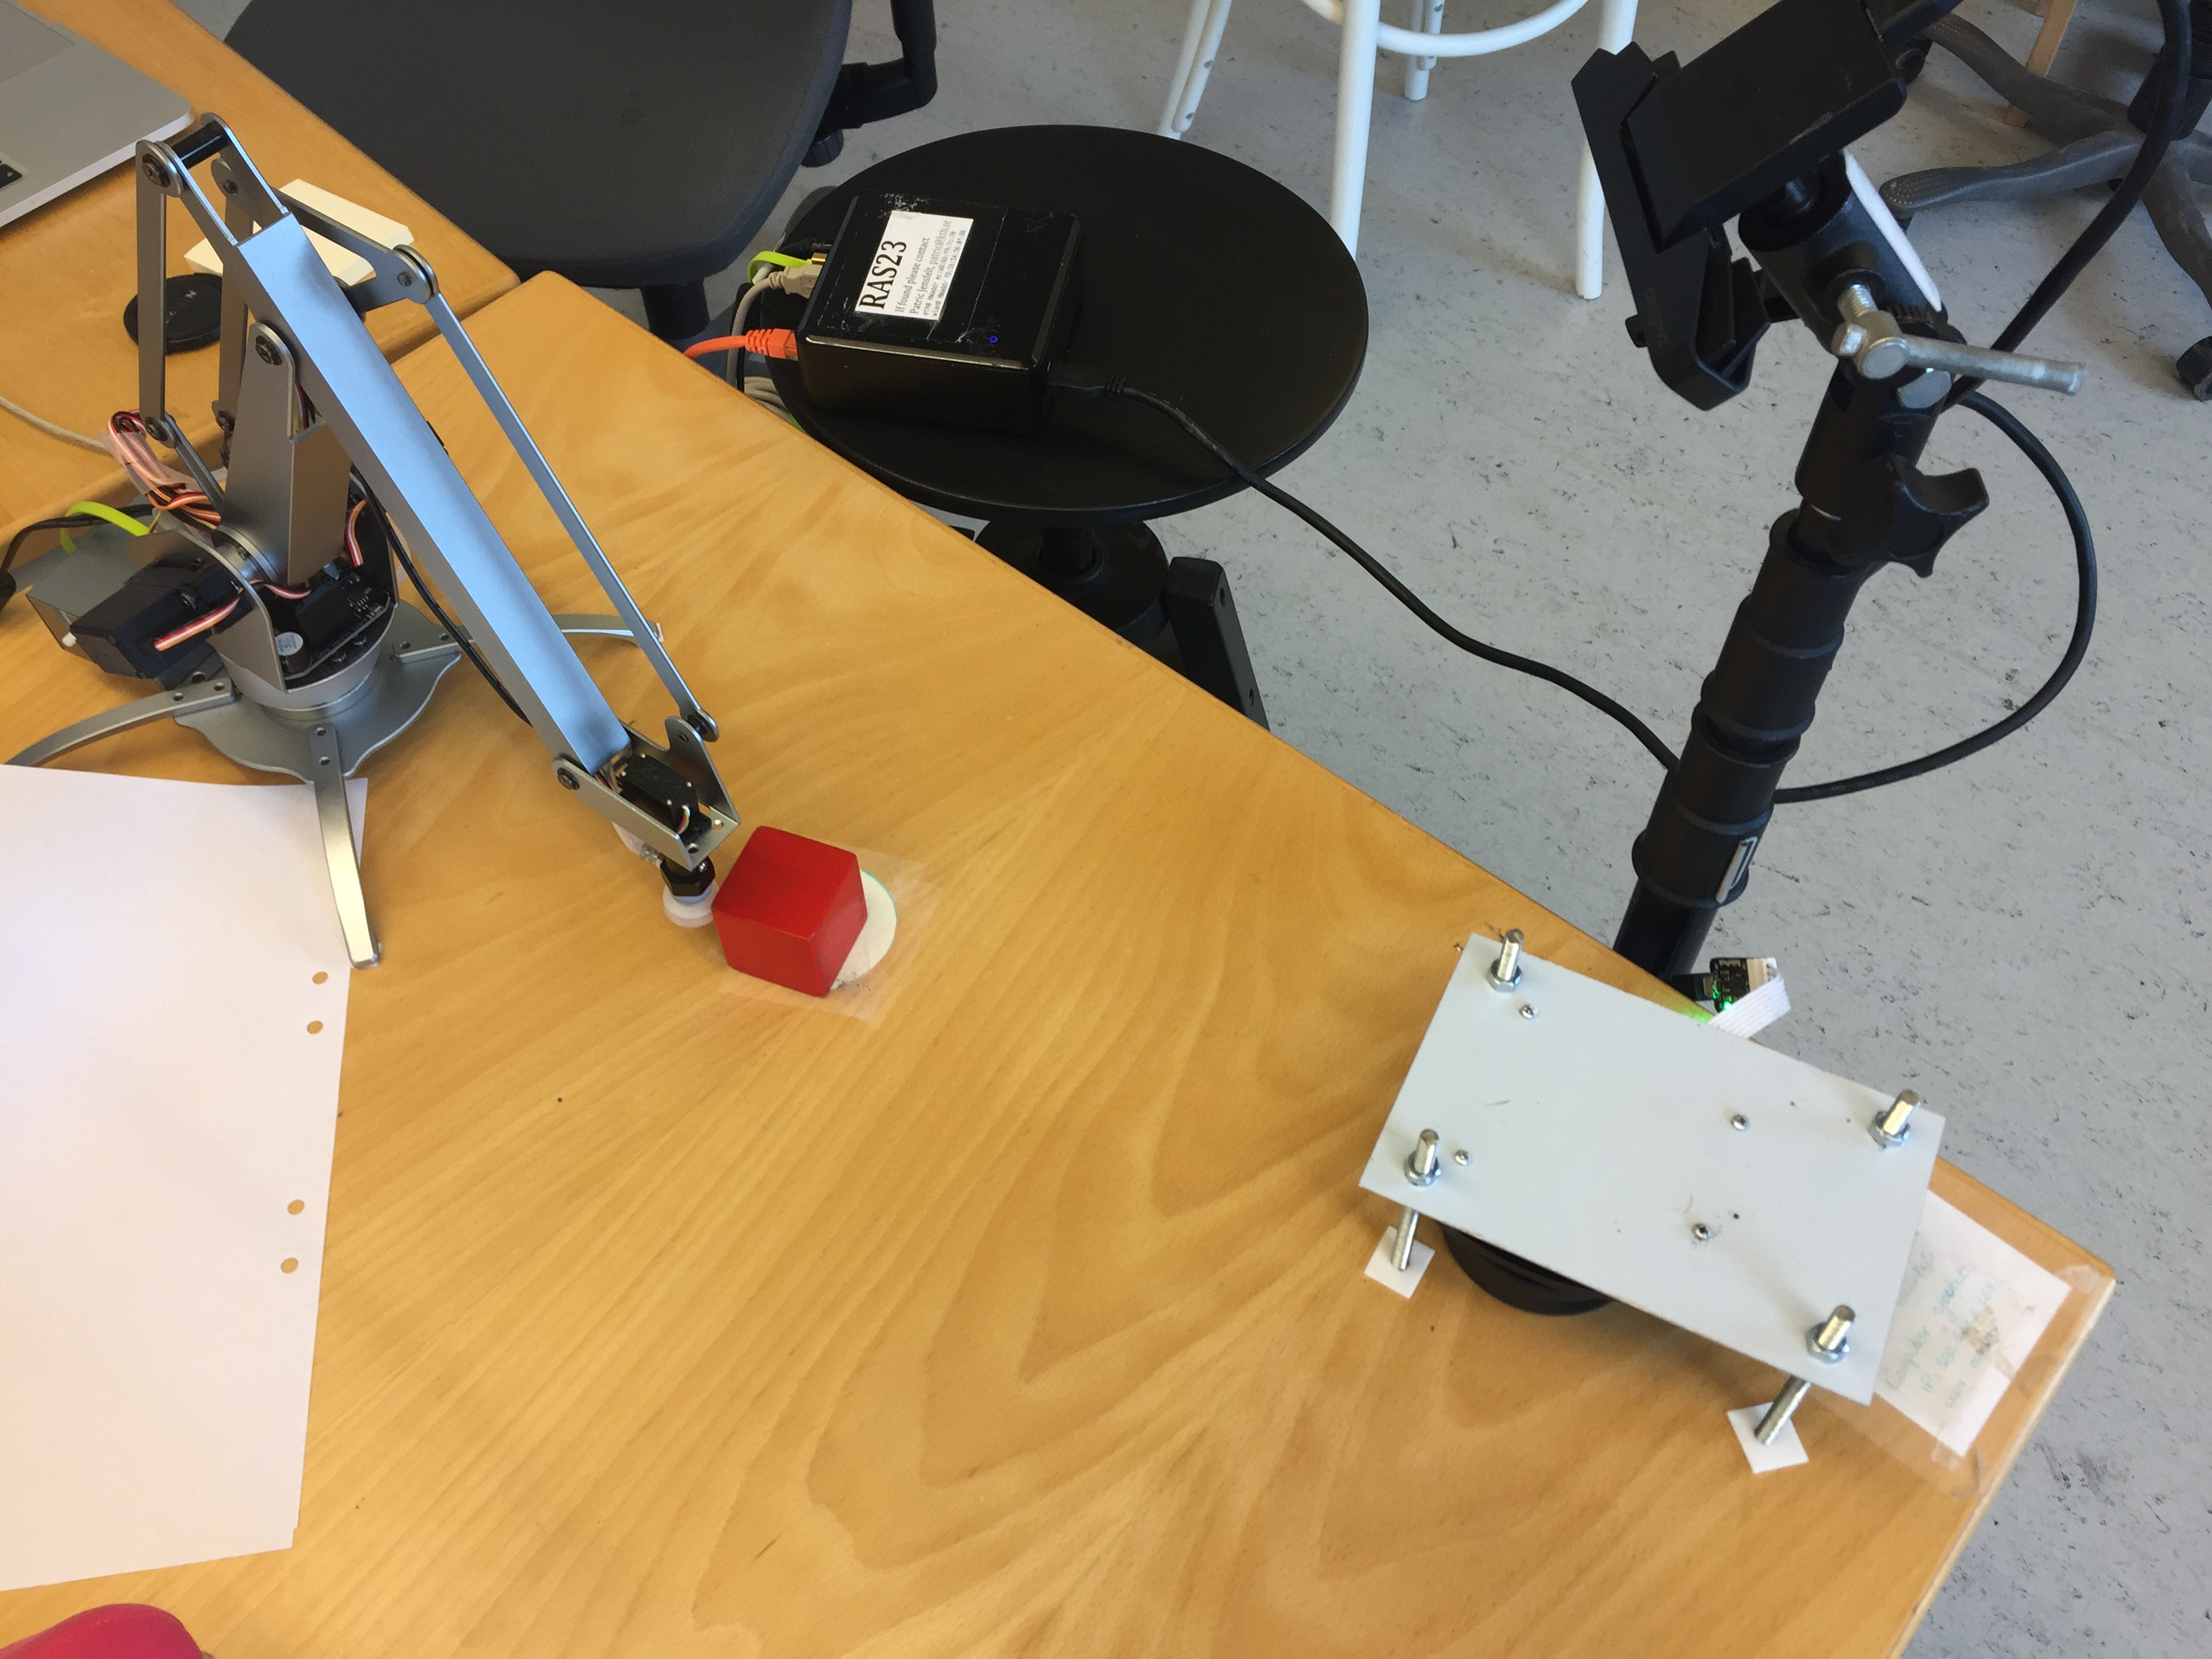
\includegraphics[width=0.48 \textwidth]{res/camera_placement_fixed.jpg}

    \caption{LIDAR seen on the right side in the picture measuring positions of
    the cube. The camera is not used in this experiment.}

    \label{fig:eef-frame}
    
\end{figure}

\section{Results}

The policy trained in simulation successfully pushes the cube towards a goal
set in the center of the workspace, video of this can be seen here:
\url{https://youtu.be/82XNDBPbJH0}. Sometimes the policy fails to push the cube
further due to small action commands not affecting the robot, and due to
differences in the shapes of the simulation object (circle) and the cube.
Adding a small noise term alleviated these problems and was used in the linked
video.
